\section{Theory}
\label{sec:theory}

\paragraph{T-A (Scorer Sensitivity Model).} $A^\ast$ is identified up to the
box $B$; sharp bounds via 4-corner evaluation when $B$ does not straddle
$\alpha+\beta=1$, and via the feasible-region supremum (proven to diverge to
the full $[0,1]$) when it does. Class B (direct adaptation of classical
misclassification bounds).

\paragraph{T-H (Sharpness).} The identified set computed by 4-corner
evaluation (non-straddling case) is exact, not an outer bound---a
linear-fractional-function vertex-theorem argument. Class B. Illustrated in
Figure~\ref{fig:identified-set}: the sharp interval is exactly the pointwise
envelope of the four corner curves across the range of observed accuracy.

\begin{figure}[t]
  \centering
  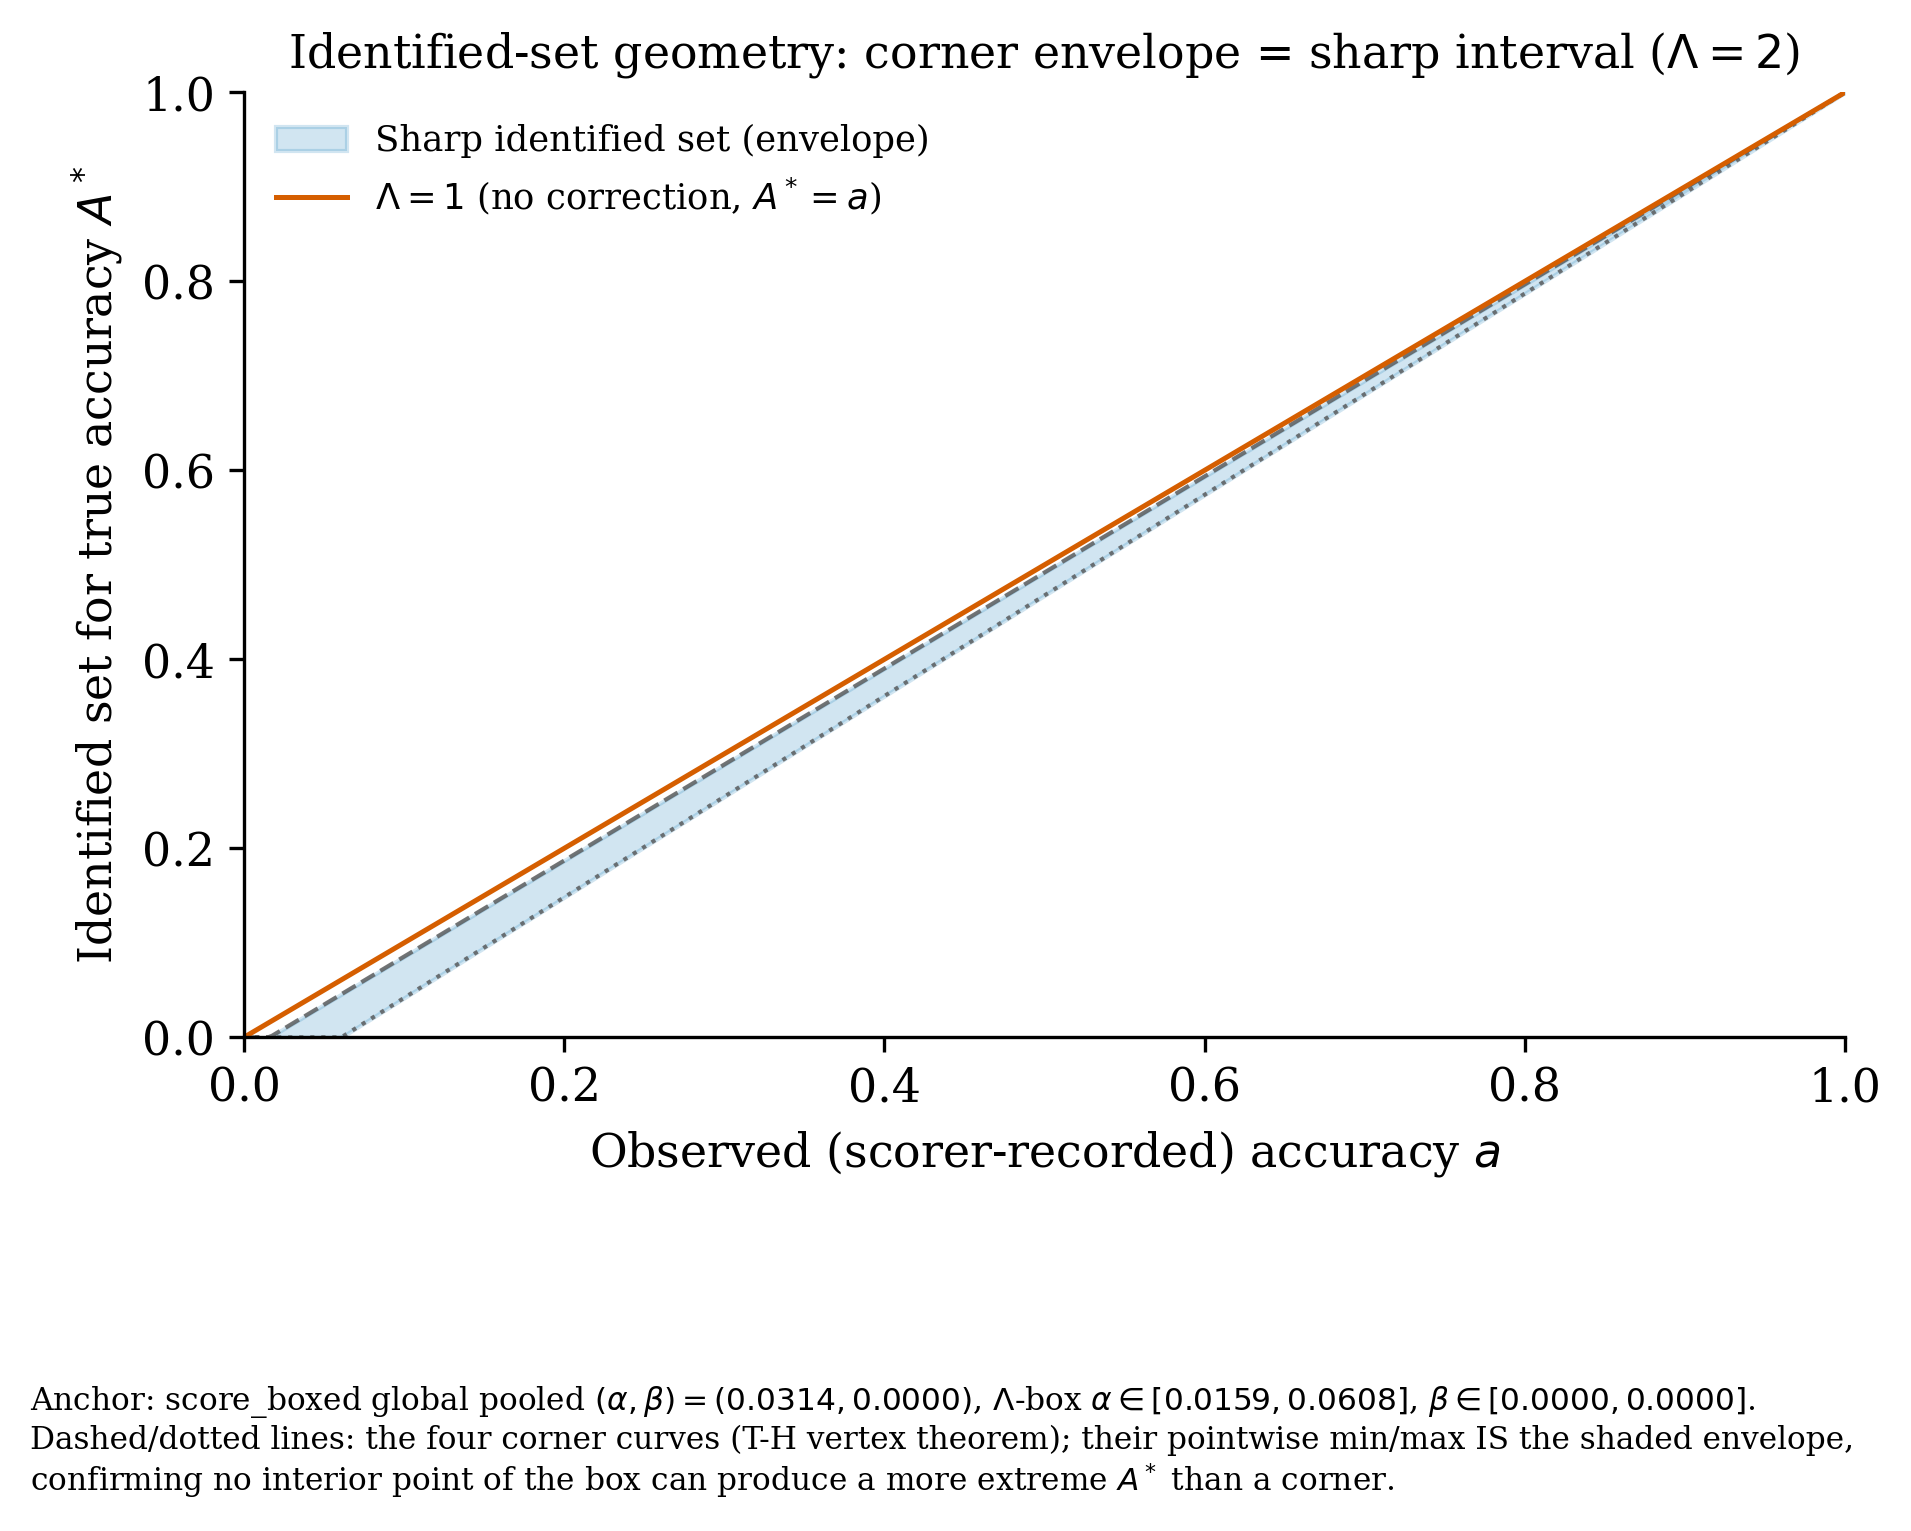
\includegraphics[width=0.62\linewidth]{fig3_identified_set_geometry.png}
  \caption{Identified-set geometry (T-H): the sharp interval is the pointwise
  envelope of the four corner curves of the $\Lambda$-box, confirming no
  interior point of the box produces a more extreme $A^\ast$ than a corner.}
  \label{fig:identified-set}
\end{figure}

\paragraph{Ranking-preservation theorem.} The ranking $A_1^\ast > A_2^\ast$
holds for every $(\alpha,\beta) \in B$ \textbf{if and only if}
$0 \notin \Delta^\ast(B)$---a direct, exact corollary of T-H's sharpness,
stated as an operational theorem because it clarifies that sharpness (not
merely conservatism) is what makes the field's existing \code{contains\_zero}
check a valid necessary-and-sufficient robustness test, not just a
sufficient one. Class B.

\paragraph{T-B (Design-sensitivity impossibility).} There exists a compound
sensitivity level $\tilde{\Lambda}$ beyond which a comparison is
unidentifiable at \emph{any} benchmark sample size---a Rosenbaum-style
design-sensitivity result \citep{rosenbaum2004design} adapted to this
setting. Class B.

\paragraph{Correlated scorer error.} Under a one-factor (shared
item-difficulty) model---the same structural assumption underlying
Dawid--Skene \citep{dawid1979maximum}---non-differential item-heterogeneity
strictly \emph{reduces} the variance of a pairwise difference relative to an
independence assumption ($\mathrm{Cov} \geq 0$, closed form, verified by
simulation to within Monte Carlo tolerance); differential loading (a
model-specific interaction with item difficulty) breaks this cancellation
and is exactly what the framework is built to bound. Class B.

\paragraph{Imperfect human reference (T-D).} A full latent-class treatment
\citep{hui1980estimating} is not justified by this paper's data (14-item
three-way rater overlap, insufficient to identify 4 rater-specific
parameters plus a prevalence)---an explicit, evidenced decision, not a
shortcut. A sensitivity bound $q_{\max}(\eta)$ is derived instead: given the
observed apparent disagreement rate and an assumed human-labeler error rate
$\eta$, the bound on the true scorer-wrong rate $q$ this could be masking. On
our audit's real data (0/69 apparent disagreements in the second, targeted
round), the bound does not have a concerning breakdown point for realistic
$\eta$ (0--5\%). Class B/C.

\paragraph{Verification-bias formalization (T-E).} The audit's
stratified-on-scorer-outcome design is checked against, not assumed to
match, the classical verification-bias structure; shown formally distinct
because the stratum-conditional sampling probability $\pi_h$ is known by
design, which is exactly the condition under which the Horvitz--Thompson
estimator \citep{horvitz1952generalization} is unbiased---proved, with the
one load-bearing assumption (no dependence on unrecorded information) named
explicitly. Class B.

\paragraph{Flip-budget uncertainty.} The flip budget $d^\ast$ (minimum
differential-error perturbation to put a comparison's sign in doubt) is
given a bootstrap confidence treatment (joint resampling of benchmark and
audit items) rather than reported as a bare point value. On the current real
MATH-Hard roster's most fragile and most robust identified pairs, $d^\ast$
is bootstrapped with 95\% intervals excluding zero cleanly in both cases
(Section~\ref{sec:results}). A rigorous asymptotic-coverage proof for this
specific nonlinear, possibly-empty-set estimand is flagged as open, not
attempted here.

\paragraph{Partial pooling.} Empirical-Bayes shrinkage toward a global
anchor genuinely propagates a local audit's effect to un-audited
models---verified directly on real data, both a benefit (stabilizes thin
per-model audits) and a documented cost (this paper's own audit-design work:
naive plug-in Neyman allocation, which implicitly relies on the raw per-cell
rate as a planning estimate, is \emph{dominated by uniform allocation} when
most cells have near-zero raw counts---Section~\ref{sec:audit-design}).
Class B/C.

\paragraph{Novelty summary.} No individual result above rises above class C
(nontrivial combination/extension); several are B (direct, correctly-cited
adaptations). The claimed contribution is the \emph{combination}---benchmark
comparison + scorer misclassification + partial identification +
audit-estimation uncertainty + audit-budget design + (secondarily)
scorer-choice dependence---evidenced with real data throughout, not the
individual mathematical pieces. See Table~\ref{tab:theory-summary} and the
full A/B/C/D classification in the supplementary novelty audit
(Appendix~\ref{sec:appendix-novelty}).

\begin{table}[t]
  \centering
  \caption{Theoretical results summary.}
  \label{tab:theory-summary}
  \small
  \begin{tabular}{@{}p{3.1cm}p{7.3cm}c@{}}
    \toprule
    Result & Statement & Class \\
    \midrule
    T-A (SSM) & Odds-ratio $\Lambda$-bounded sensitivity family for $(\alpha,\beta)$ & B \\
    T-H (sharpness) & Identified interval = corner envelope, $\cap\,[0,1]$ & A/B \\
    T-B (design sensitivity) & $\tilde\Lambda$ at which a comparison first becomes unresolved & B \\
    Correlated-error bound & Propositions bounding shared-scorer-error correlation's effect & C \\
    T-D (imperfect reference) & $q_{\max}(\eta)$ bound under a non-omniscient human reference & C \\
    T-E (verification bias) & HT validity under disproportionate audit sampling & A/B \\
    Ranking-preservation & Exact sign-flip condition, corollary of T-H & C \\
    Flip-budget uncertainty & Bootstrap CI for the minimum sign-flipping perturbation & C \\
    Neyman allocation & Classical; found \emph{dominated} by proportional on real sparse data & A + empirical (C) \\
    \bottomrule
  \end{tabular}
\end{table}
